\chapter{The what, and the why}\label{chap:chap1}

\epigraph{``Simplicity is a great virtue but it requires hard work to achieve it and education to appreciate it. And to make matters worse: complexity sells better.''}{\textit{Edsger W. Dijkstra} -- EWD896}

\paragraph{}
In this chapter we will provide a brief introduction to the LEGv8 ISA, together with a survey of its publicly available simulators. After that, we will focus on the simulator chosen for this thesis' work, namely Arm's, by giving an overview of its codebase, design choices, advantages, and shortcomings. The chapter will end with a summary of the motivations for choosing to work on this specific simulator. 

\section{What is an ISA?}

\paragraph{}
A computer is a device which is capable of processing, storing, and displaying information \cite{computerdefweb}.
It is clear from this definition that, when deciding how to design and build a computer, one must at least take into consideration the way data is 
stored and organized (i.e., the memory), and the mechanisms through which the computer is able to manipulate said data (i.e., the processor).
As per the definition, the concept of a computer does not impose a certain technological choice to its physical realization. Nonetheless, the vast majority of computers nowadays
are built through the assembly of digital components and thus natively speak the language of the binary number system.
As such, just like a user operating a mechanical device needs to interact with the physical parts of the system,  dealing with a computer at this physical level
would require the programmer to manually insert ones and zeros into the right places for it to perform its computations.
Such an operation would require an intimate knowledge of the physical realization of the computer, and even minimal
changes to its internal components might jeopardize the correctness of any program written for an earlier version.
\paragraph{}
Early on in the history of computers it was understood that an additional layer of abstraction was needed in order to separate the hardware from the software
and give more freedom both to the designers of the computers, and the programmers operating on them. This layer of abstraction is called an Instruction Set Architecture,
which from now on will be called ISA for short. An ISA provides a logical specification of how a computer manages its memory and what the instructions that is
capable of performing are. This forms the layer through which all software must interface with in order to interact with the hardware.

\section{What is LEGv8?}

\paragraph{}
The ISA focus of this thesis is the LEGv8 ISA, an ARM-inspired architecture created by David A. Patterson and John L. Hennessy and designed to serve as a teaching
tool in their book \emph{Computer Organization and Design (ARM Edition)} \cite{patterson2016computer}.  Quoting the authors:
\paragraph{}
\emph{``The choice of instruction set architecture is clearly critical to the pedagogy of a
computer architecture textbook. We didn’t want an instruction set that required
describing unnecessary baroque features for someone’s first instruction set, no
matter how popular it is.
Given the growing popularity and the simple elegance of the MIPS instruction
set, we switched to it for the first edition of this book and to later editions of the
other book. MIPS has served us and our readers well.
The incredible popularity of the ARM instruction set led some instructors to ask for a version of the book based on
ARM. Although ARMv8 is much, much larger than MIPS we found a subset of ARMv8
instructions that is similar in size and nature to the MIPS core used in prior editions,
which we call LEGv8 to avoid confusion. Hence, we wrote this ARMv8 edition.''} pp. xvi-xvii
\paragraph{}
Although the authors refer to LEGv8 as a ``subset'' of ARMv8, it is important to note that, in fact, some additions and changes have been made to the instruction set to simplify it further and make it more coherent for pedagogical purposes. This results in LEGv8 code not being executable on an ARM-compatible computer but instead requiring some manual translation. This, together with the purely academic nature of the ISA, means that no LEGv8-compatible computers are commercially available and all LEGv8 code must be executed through a software simulation or somehow converted to the ARMv8 equivalent.

\section{Overview of the LEGv8 ISA}

\begin{figure}[H]
	\centering
	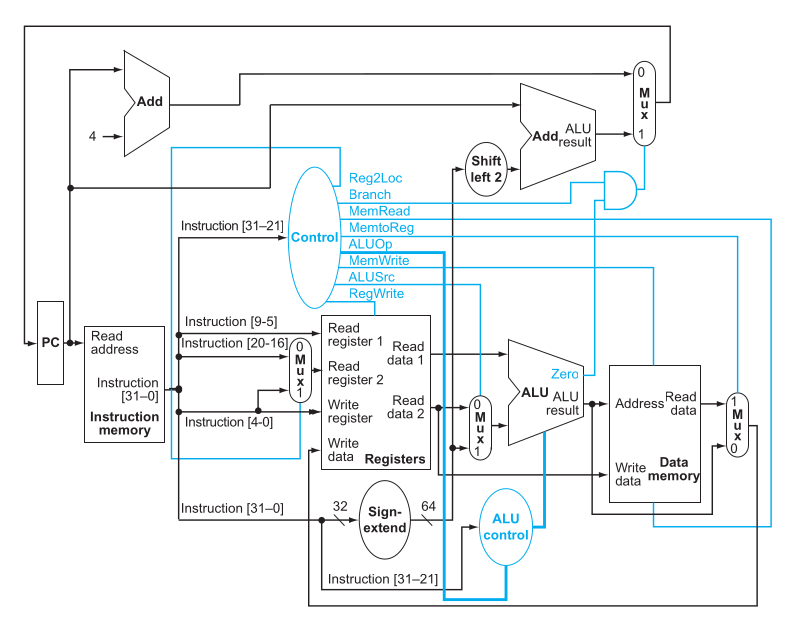
\includegraphics[width=1\textwidth]{img/legv8_logical_scheme.png}
	\caption{The logical scheme of the LEGv8 architecture. From \emph{Computer Organization and Design (ARM Edition)} \cite{patterson2016computer} p. 277}
 \label{fig:legv8logicdiag}
\end{figure}

\paragraph{}
In the book \cite{patterson2016computer}, the LEGv8 ISA is specified with two different levels of abstraction. Throughout the whole text, a high level description of the ISA is provided and utilized, and it will be the one summarized in the rest of this section. This specification contains the entire LEGv8 instruction set, but doesn't concern itself with the lower level design needed to create a working implementation. In Chapter 4 of the book, the authors aim to provide a closer description of a model LEGv8 processor following the scheme depicted in Figure \ref{fig:legv8logicdiag}. Although the chapter goes into much more detail than the figure shown, providing a description of the entire ISA at this level would require an entire book of its own. For this reason, the authors limited themselves to a subset of LEGv8 containing only a handful of integer instructions. The distinction between these two specifications will become relevant in the next sections and chapters.

\subsection{Architecture type}
\paragraph{}
As Figure \ref{fig:legv8logicdiag} makes apparent, the LEGv8 ISA follows the Harvard architecture model \cite{harvardarchweb}.  This means that the memory is logically divided in two: the \emph{instruction memory} to store the code of the program, and the \emph{data memory} to store the data necessary to the program during its execution. These two memory sections are addressed separately.
\subsection{Registers}\label{chap:chap1registers}
\paragraph{}
Registers are the memory components that the processor uses to temporarily store the data it needs to perform its operations. They are few, fast, and expensive, and are independent from the main memory.\\
LEGv8 defines 32 64-bit \verb|X| registers for storing integer values and memory addresses and 32 64-bit \verb|D| registers for storing double precision floating point values. This makes LEGv8 a 64-bit ISA. There are also 32 32-bit \verb|S| registers dedicated to single precision floating point values, albeit being purely logical and simply occupying the lower 32 bits of the \verb|D| registers. Unlike ARMv8, the presence of 32-bit \verb|W| integer registers is not contemplated.\\
LEGv8 also defines a convention for using the registers, which, while not being entirely enforced by the hardware, is to be followed when writing any non-trivial program. It also specifies some alternative names with which to refer to certain registers for ease of readability. Figure \ref{fig:legv8intregconv} shows the convention for integer registers, but there are analogous conventions for the floating point ones too.
\begin{figure}[H]
	\centering
	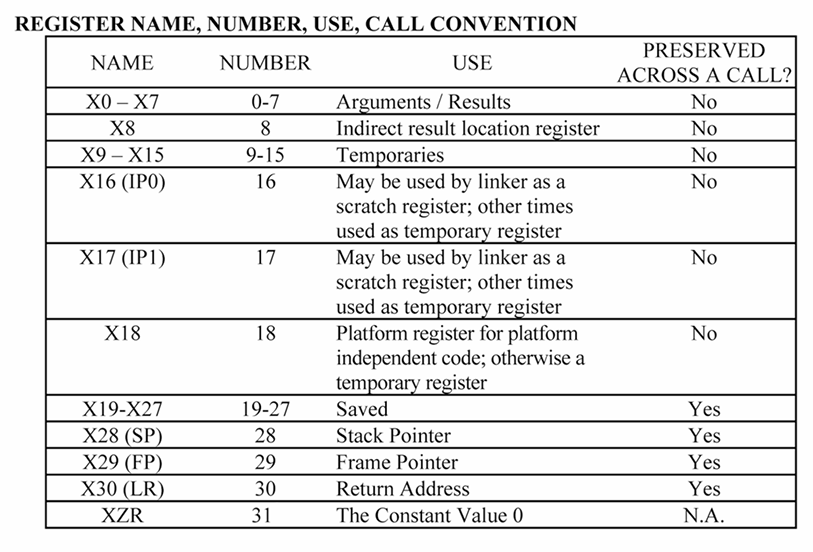
\includegraphics[width=1\textwidth]{img/registers_conventions.png}
	\caption{Integer registers usage convention. From \emph{Computer Organization and Design (ARM Edition)} \cite{patterson2016computer}.}
 \label{fig:legv8intregconv}
\end{figure}

In addition to the normal registers directly accessible by the programmer, more exist to store the \emph{program counter (PC)} (i.e. the address of the current instruction to be executed) and various flags that keep track of overflows or carry bits in arithmetic operations and comparisons.
\paragraph{Condition flags}
The registers responsible for holding the condition flags are of vital importance when needing to perform comparisons both in the case of signed and unsigned integer values. Here are the conditions that the four flag registers follow, as explained in Patterson's text \cite{patterson2016computer} on page 97:
\begin{itemize}
    \item negative (N) – the result that set the condition code had a 1 in the most
significant bit;
\item zero (Z) – the result that set the condition code was 0;
\item overflow (V) – the result that set the condition code overflowed; and
\item carry (C) – the result that set the condition code had a carry out of the most
significant bit or a borrow into the most significant bit.
\end{itemize}

\subsection{Memory}
\paragraph{}
While in practice LEGv8 follows the Harvard model by addressing each section separately, its two memories can be logically stitched together as a single array of bytes, with each memory address referring to one of said bytes. This unified logical representation of the memory is divided into 5 parts as depicted by Figure \ref{fig:legv8memdiag}: a \emph{reserved} segment for internal usage, a \emph{text} segment containing the program code (and from which the program counter starts), a \emph{static data} segment containing the constants defined at compile time, and a \emph{dynamic data} and \emph{stack} segments sharing the same location of memory. The \emph{stack} memory starts at the address defined by the \emph{stack pointer (SP)} and grows downwards. It is the memory that gets allocated when calling functions, and it contains all the data therein utilized for the sole duration of their execution. Each function allocates its portion of the stack, called \emph{stack frame}, and it should be the only one it accesses. The \emph{dynamic data}, or \emph{heap}, begins immediately after the \emph{static data} segment and grows upwards. It contains the dynamically allocated data of the program, thus its size depends on a particular execution of the program and cannot be predicted beforehand. This segment contains the shared data of the program, which can be accessed from everywhere.
\begin{figure}[H]
	\centering
	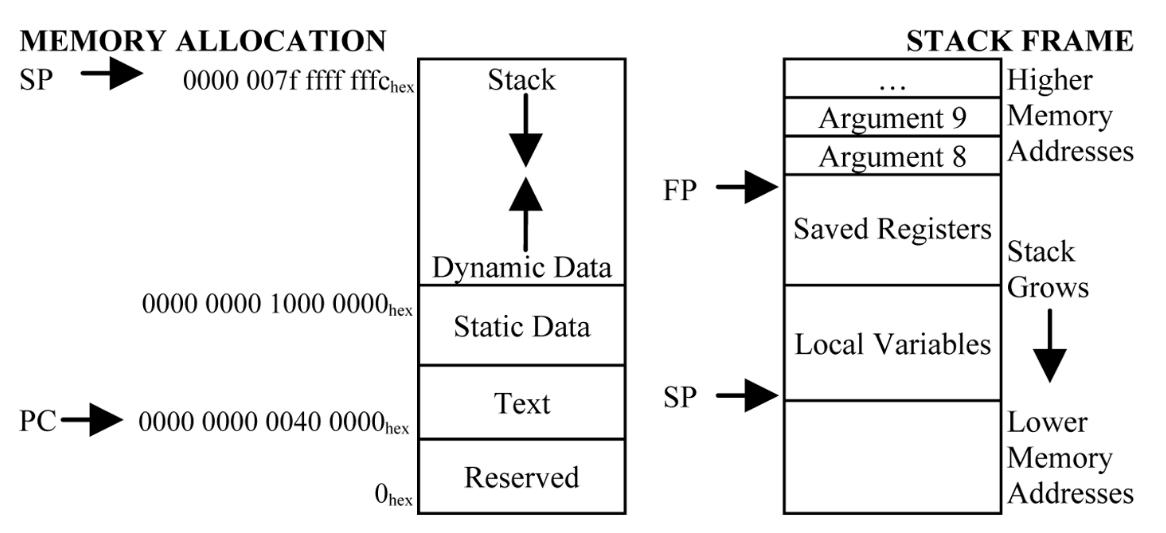
\includegraphics[width=.8\textwidth]{img/main_memory_layout.png}
	\caption{Logical division of the memory. From \emph{Computer Organization and Design (ARM Edition)} \cite{patterson2016computer}.}
 \label{fig:legv8memdiag}
\end{figure}
\subsection{ALU}
\paragraph{}
The ALU is the component responsible for all the arithmetical operations inside of the processor. The LEGv8 ALU is capable of performing 64-bit integer operations and both single and double precision floating point operations. Hybrid operations between different types of data or registers are not possible. As shown in Figure \ref{fig:legv8logicdiag}, the type of operation that the ALU is expected to perform and some additional configuration is provided by the control unit through an ALUop code.
\subsection{Pipeline}
\paragraph{}
Among the eight great ideas in computer architecture compiled by the authors in the book, a particular kind of  parallelism, called \emph{pipelining}, is mentioned.
\emph{Pipelining} refers to the ability of a computer architecture to organize its instructions and its structure in a way that makes it possible to overlap their execution without waiting for the completion of each to begin the next. The execution of only one instruction at a time is called \emph{single cycle} execution. LEGv8 achieves pipelining by splitting the execution of an instruction into 5 stages: \emph{fetch}, \emph{decode}, \emph{execute}, \emph{data access}, and \emph{write back}, with the order shown in Figure \ref{fig:legv8pipeline}.\\
As the names suggest, the \emph{fetch} stage is responsible for acquiring instructions from the instruction memory, the \emph{decode} stage decodes the instructions, reads the registers involved in the operation, and configures the control unit accordingly, the \emph{execute} stage performs the actual computation through the ALU, the \emph{data access} stage is responsible for accessing the data memory, and the \emph{write back} stage writes the result of the operation into the registers.
\begin{figure}[H]
	\centering
	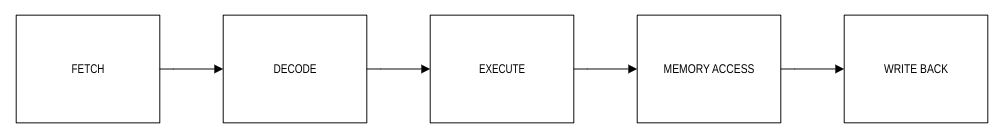
\includegraphics[width=1\textwidth]{img/5_stage_pipeline.png}
	\caption{The 5 pipeline stages}
        \label{fig:legv8pipeline}
\end{figure}
As an example, suppose that two instructions do not make use of shared resources. If one is being decoded why can't the next one get fetched in the meantime? And if one is accessing the memory, why can't the other perform its computation via the ALU at the same time? This is, of course, a simplistic example, and in many situations subsequent instructions get in the way of each other by making use of the same registers or memory locations, and as such create an implicit order of execution that needs to be followed if we want to obtain correct results.
Not all instructions make use of all the pipeline stages and this is taken into consideration when optimizing the execution flow.
These situations in which instructions conflict with one another are called \emph{hazards}, and need to be dealt with by either strategically rearranging the instructions in the code to avoid such conflicts, or by making additions to the architecture in order to create ``shortcuts'' that bypass the pipeline and provide the correct data to the other stages. If all else fails, which is the case for some combinations of instructions, the processor can simply stall part of the pipeline to let an instruction go through the stages without creating dependency problems. This is, of course, the least desirable option.

\subsection{Instructions}
\paragraph{}
As previously mentioned, LEGv8 can be considered a subset of ARMv8, but with a few caveats. Many higher level instructions performing aggregate or complex operations have been omitted altogether in order to keep the ISA as minimal as possible, and of the ones that have been kept, many have been revisited to make them clearer in their scope. For example, in ARMv8 the \verb|ADD| instruction can be used with both 32 and 64 bit integer registers, and with both register-based and immediate-based (i.e., defined directly in the program code) values. This of course allows the ARMv8 programmer to remember a single mnemonic (i.e., the name of an instruction) and use it in all sorts of operations, but it obscures some important underlying design differences that might be valuable to computer architecture students. In LEGv8 instead, it has been decided to split the \verb|ADD| instruction into \verb|ADD| and \verb|ADDI|, for register and immediate values usage respectively. Similarly, in ARMv8 the \verb|FADD| instruction is capable of performing additions both in the case of single and double precision registers, whereas in LEGv8 the instruction has been split into \verb|FADDS| and \verb|FADDD| for performing the operation only on single precision or double precision registers respectively. Just like ARMv8, LEGv8 too uses the IEEE-754 standard \cite{ieee754} for the representation of floating point values and the way its instructions operate on them.\\Figure \ref{fig:legv8instrlist} provides a full list of all the instructions defined by LEGv8 together with their encoding.
\begin{figure}[H]
	\centering
	\makebox[\textwidth][c]{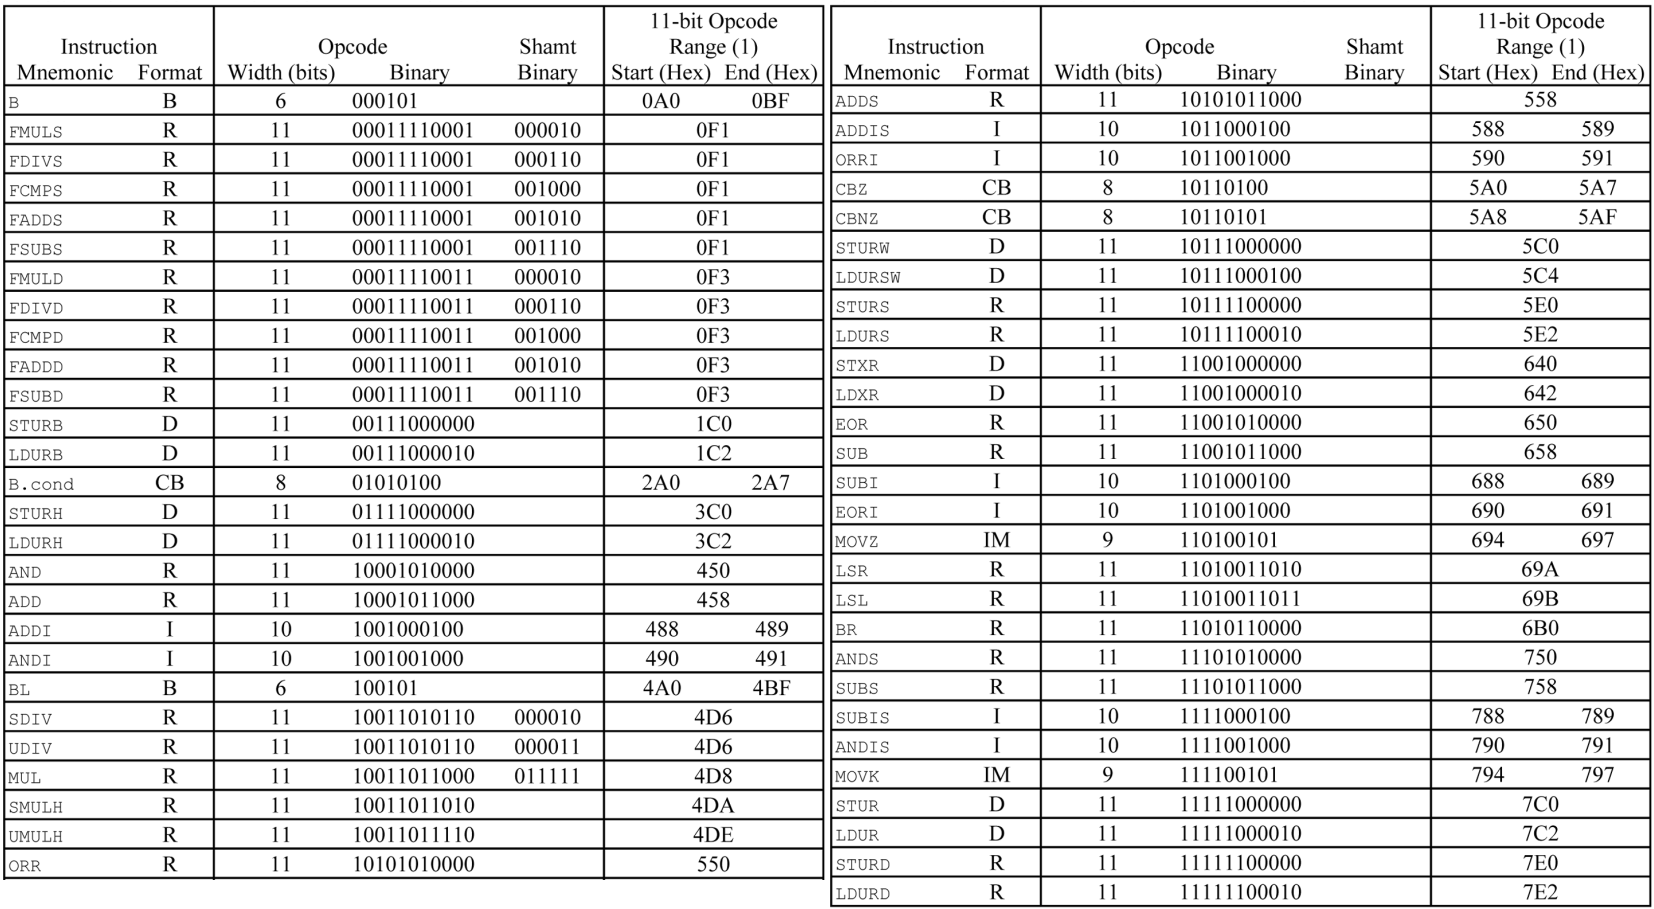
\includegraphics[width=1.0\textwidth]{img/legv8_instruction_set.png}}
	\caption{The complete LEGv8 instruction list. Adapted from \emph{Computer Organization and Design (ARM Edition)} \cite{patterson2016computer}.}
    \label{fig:legv8instrlist}
\end{figure}
As Figure \ref{fig:legv8instrencod} shows, the instructions are encoded with the same length of 32 bits in order to fetch and decode them more efficiently. They are also grouped into 6 instruction formats to give a more homogeneous encoding to operations performing similar steps and increase their decoding speed.
The \verb|R|-type instructions perform operations solely on registers, the \verb|I|-type instructions make use of immediate values, the \verb|D|-type instructions access the memory, the \verb|B|-type and \verb|CB| perform unconditional and conditional branching respectively, and the \verb|IW|-type instructions to perform MOV instructions (i.e., instructions where data is simply moved around) with wider immediate values.
\begin{figure}[H]
	\centering
	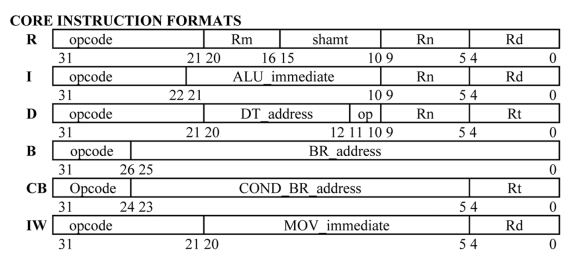
\includegraphics[width=1\textwidth]{img/instruction_types.png}
	\caption{The 6 formats of LEGv8 instructions with their encoding pattern. From \emph{Computer Organization and Design (ARM Edition)} \cite{patterson2016computer}.}
 \label{fig:legv8instrencod}
\end{figure}
\subsection{Control unit}
\paragraph{}
While everything we have talked about until now can be considered part of the \emph{datapath} of the processor, meaning the series of components the data passes through in order to complete a computation, this datapath needs an additional component to coordinate its functioning. The control unit is the component responsible for coordinating the single cycle and the pipelined datapath, configuring the various components to perform the desired operations in the correct order using the correct parameters and avoiding hazards.
\subsection{Other discrepancies between LEGv8 and ARMv8}
\paragraph{}
There are ulterior design choices that differentiate LEGv8 from ARMv8 and make them even more incompatible with one another.  We will report them for completeness, but are merely tangential to this thesis' work. Citing the authors of the book \cite{patterson2016computer} at pages 174 and 175:
\subparagraph{}
\emph{
``In the full ARMv8 instruction set, register 31 is XZR in most instructions
but the stack pointer (SP) in others. We think it is confusing, so register 31 is
always XZR and SP is always register 28 in LEGv8. If you stick to using XZR
and SP for register names when using the assembler and simulator, it should
not be a problem, but this subtle distinction might show up in visualizations
of the state of the processor, for example.''}
\subparagraph{}
\emph{
``The immediate fields for ANDI, ORRI, and EORI of the full ARMv8
instruction set are not simple 12-bit immediates that we assume in LEGv8.
ARMv8 has an algorithm for encoding immediate values as repeating
patterns. This means that some small constants (e.g., 1, 2, 3, 4, and 6) are
valid, while others (e.g., 0, 5) are not. Thus, the assembler may insert more
instructions than you might expect to create simple constants, or fewer if
you pick a lucky large constant. The official definition is the bit pattern can
be viewed “as a vector of identical elements of size e = 2, 4, 8, 16, 32, or 64
bits. Each element contains the same sub-pattern, that is a single run of 1
to ($e - 1$) nonzero bits from bit 0 followed by zero bits, then rotated by 0 to
($e - 1$) bits.” Don’t try to figure this out yourself; just leave it to the assembler!''}

\section{The LEGv8 simulators landscape}

\paragraph{}
We have already mentioned that LEGv8 is a purely academic ISA designed to serve the purposes of a single undergraduate textbook. Although more complex academic architectures have been physically realized by research groups and even gained commercial traction \cite{riscvweb}, there are currently no publicly available implementations of LEGv8 to be used to run its native instructions. This means that, for any LEGv8 code to be successfully executed, a software simulator is currently needed. Being an ISA taught at a number of universities, various simulators have been created both by students and educators to aid in their teaching or as homework requirements. For this reason, the vast majority of simulators are limited in their scope and aim to implement only a subset of the LEGv8 ISA.

\subsection{The survey}

\paragraph{}
The current offering of publicly available LEGv8 simulators can be divided into two categories: simulators that aim to reproduce the lower level design presented in the textbook \cite{patterson2016computer}, in Chapter 4, and the simulators providing a high level simulation of the instruction set as described in the previous section.
\paragraph{Methodology}
GitHub \cite{githubweb} was chosen as the public repository in which to perform the survey. The keywords used to identify possible simulators were ``LEGv8'' and ``simulator''. Simulators with lacking documentation or which were described by the author(s) as partially done or not working were excluded. The simulator chosen for this thesis was also excluded to better highlight its features in the following sections.

\newpage
\begin{landscape}
\begin{table}[H]
	\centering
            \resizebox{1.5\textwidth}{0.2\textwidth}{\begin{tabular}{|c|c|c|c|c|c|c|}
		\hline
		\textbf{Repository} & \textbf{Language} & \textbf{Integer Support} & \textbf{Pipelined} & \textbf{Registers view} & \textbf{Stack view} & \textbf{Floating Point Support} \\
		\hline
		\url{https://github.com/lcpckp/leg-cpu-sim} & Java & Partial & No & Yes & Yes & No \\
		\hline
		\url{https://github.com/chrwoods/legv8-emul} & C/C++ & Partial & Yes & Yes & Yes & No \\
		\hline
		\url{https://github.com/mtalyat/LEGv8Day} & C\# & Partial & No & Yes & Yes & No \\
		\hline
		\url{https://github.com/eaxworthy/LegV8Interpreter} & Python & Partial & No & Yes & Yes & No\\
		\hline
		\url{https://github.com/AdinAck/LEGv8-Simulator} & Swift & Partial & No & Yes & Yes & No \\
		\hline
		\url{https://github.com/anvitha305/legv8sim} & Python & Partial & No & Yes & Yes & Double precision only \\
		\hline
		\url{https://github.com/dangbandy/LegV8-Simulator} & C++ & Partial & No & Yes & Yes & No\\
		\hline
		\url{https://github.com/schang412/LEGv8-PyEmu} & Python & Partial & No & No & No & No\\
		\hline
		\url{https://github.com/GeorgePerreault/LEGV8_Interpreter} & Python & Partial & No & Yes & Yes & No\\
		\hline
	\end{tabular}}
	\caption{The surveyed software simulators}
        \label{tab:softsims}
\end{table}

\begin{table}[H]
	\centering
	\resizebox{1.5\textwidth}{0.2\textwidth}{\begin{tabular}{|c|c|c|c|c|c|c|}
		\hline
		\textbf{Repository} & \textbf{Language} & \textbf{Integer Support} & \textbf{Pipelined} & \textbf{Floating Point Support} \\
		\hline
		\url{https://github.com/nxbyte/ARM-LEGv8} & Verilog & Partial & Yes & No \\
		\hline
		\url{https://github.com/phillbush/legv8} & Verilog & Partial & Yes & No \\
		\hline
		\url{https://github.com/ronitrex/ARMLEG} & Verilog & Partial & Yes & No \\
		\hline
		\url{https://github.com/mattco98/LEGv8-Processor} & Verilog & Partial & Yes & Partial \\
		\hline
		\url{https://github.com/amaurilopez90/LEGv8-CPU} & Verilog & Partial & Yes & No \\
		\hline
		\url{https://github.com/miguelangelo78/LEGv8-ISA} & Verilog & Partial & Yes & No \\
		\hline
		\url{https://github.com/brianworts/LEGv8_SingleCycle_Processor} & Verilog & Partial & Yes & No \\
		\hline
		\url{https://github.com/egflo/LEGv8} & Verilog & Partial & Yes & No \\
		\hline
		\url{https://github.com/ad153153/LegV8} & Verilog & Partial & Yes & No \\
		\hline
	\end{tabular}}
	\caption{The surveyed hardware simulators}
        \label{tab:harsims}
\end{table}
\end{landscape}
\newpage

\subsection{Software simulators}
\paragraph{}
The surveyed software simulators in Table \ref{tab:softsims} are in line with the previously made remarks. They are written in high level languages such as Java, C++, C\#, Swift, and Python, and take the high level approach to LEGv8 as described near the beginning of the chapter. They do not implement the entirety of the integer arithmetic, although on average they include more instructions than hardware simulators. The languages they are written with allow most of them to provide a visualization of the registers and the stack to the user, in some cases through a GUI. Only one of them simulates the LEGv8 pipeline, and only one includes floating point arithmetic, although just the double precision one.

\subsection{Hardware simulators}
\paragraph{}
These simulators concern themselves with implementing the lower level description of LEGv8, as such all of them use a hardware description language. Of all of the surveyed ones, Verilog is the only one used. Because of this, they cannot provide any human-readable representation of the internal state of the simulation, thus visualization options weren't included in the fields of the table. Because they closely follow the design as presented in the book, they only implement a few integer instructions total, but on the other hand all of them are pipelined. Only one furthers its design by including some floating point operations.

\subsection{Conclusions}
\paragraph{}
It is clear from this brief survey that the LEGv8 simulators space lacks any desirable candidates for code execution and inspection, as the software simulators are incomplete and platform-dependant, and the hardware ones are extremely limited in their scope, and lack interactivity and comprehensive visual output capabilities. Furthermore, most of them are finished projects and are not currently being maintained or expanded.

\section{Arm's LEGv8 simulator} \label{chap:chap1simoverview}
\paragraph{}
Among the surveyed simulators, an important entry is missing. Indeed, when searching for a ``LEGv8 simulator'' both on GitHub and through various search engines, the first results all refer to a project \cite{legv8simARMrepo} developed and released officially by Arm. From this metric we can infer that this is in fact the most prominent publicly available LEGv8 simulator, at least regarding authority and sheer exposure. In this section we will provide an overview of the simulator from the user's and the developer's perspectives, and in both cases detailing its strong points and shortcomings.

\subsection{Obtaining the simulator}
\paragraph{}
The project is currently hosted on a public GitHub repository \cite{legv8simARMrepogit} published by the account Arm Education. The source code and the resulting application are not clearly separated into different packages. Instead, both users and developers can download the entire project either by cloning the repository through \verb|git| \cite{gitweb} or by downloading a prepackaged release from the Releases section of the web page. This version differs from the source code only by some minor updates to the project's license and \verb|README| files. Nested inside of the downloaded folder, the source code is placed under \verb|/src|, and the executable web application under \verb|/war|.

\subsection{An outside look}\label{chap:chap1outsidelook}
\paragraph{}
Here we will present the contents of the UI of the simulator together with a typical workflow from the user. At the end, a critical look of this experience will be provided.
\subsubsection{The look and feel}
\paragraph{}
The simulator presents itself as a web application. It is launched by opening the \verb|LEGv8_Simulator.html| file with a web browser and the user is presented with the UI shown in figure \ref{fig:ogsimhomepage}.
\begin{figure}[H]
    \centering
    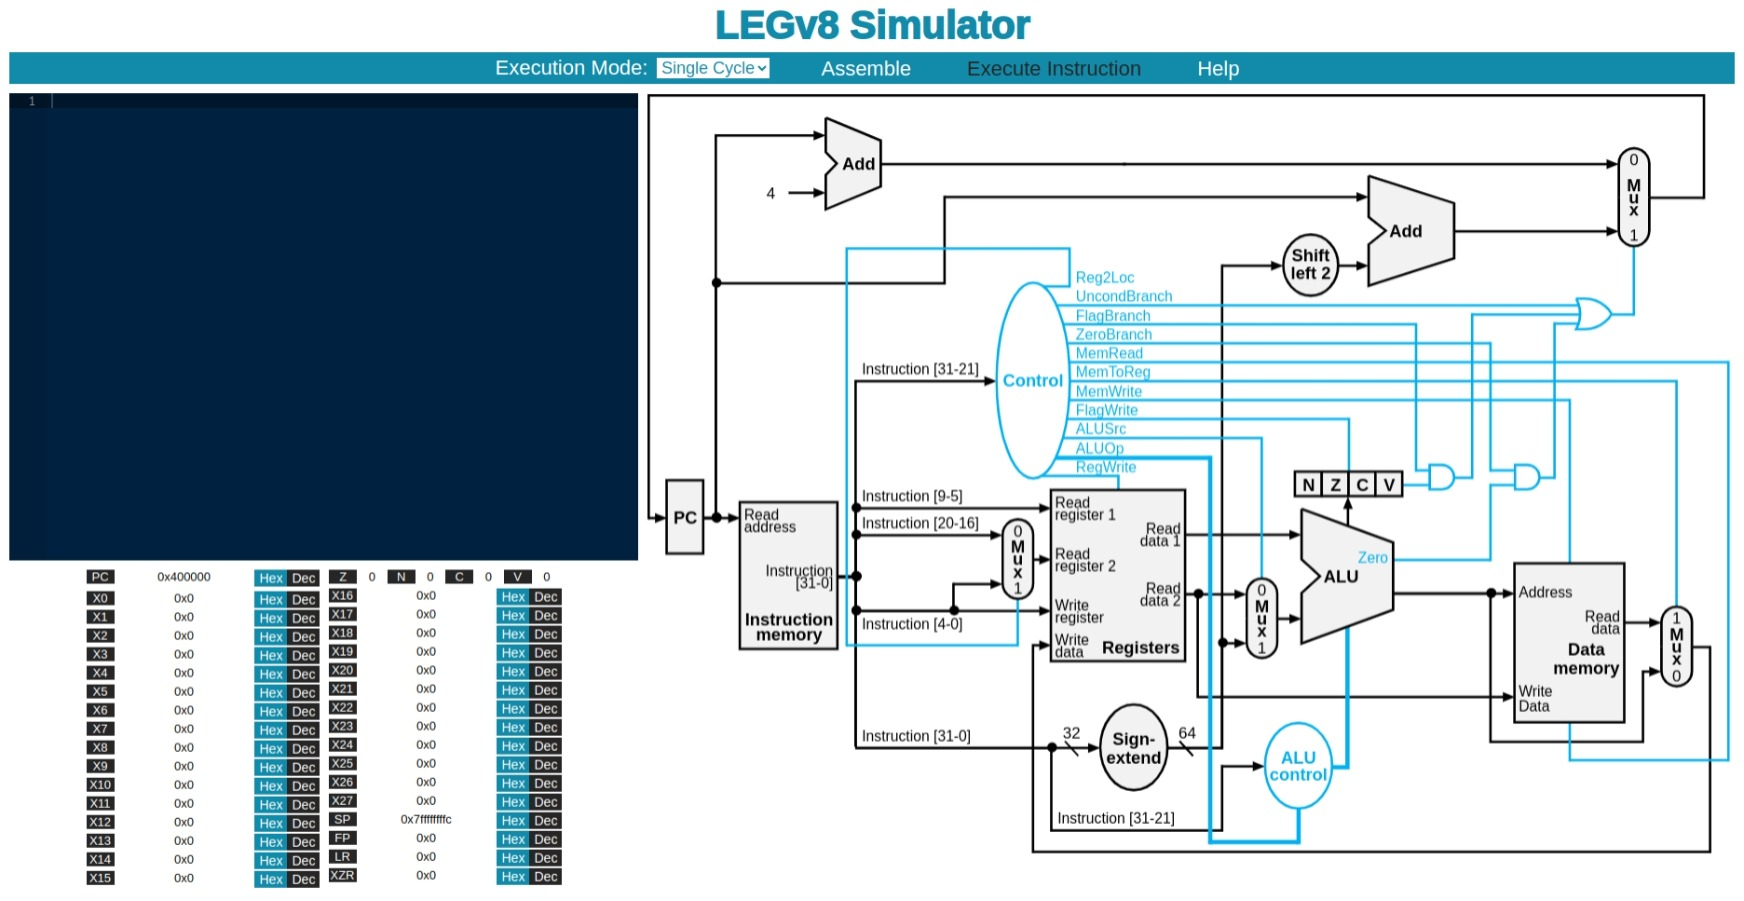
\includegraphics[width=1\linewidth]{img/old_single_cycle.jpeg}
    \caption{The simulator's home page}
    \label{fig:ogsimhomepage}
\end{figure}
At the top of the page stands a menu bar consisting of four elements. The first three pertain to the simulator's code execution and their effect is limited to the current page, while the last one, bearing the label \emph{Help}, redirects the user to a page containing both a tutorial for the application and a brief overview of LEGv8.
\subparagraph{}
The \emph{Execution Mode} selector allows the user to choose between a single cycle simulation and a pipeline simulation. These two modes present slightly different UIs, with the former being shown in Figure \ref{fig:ogsimhomepage} and the latter in Figure \ref{fig:ogpipelineview}.
\begin{figure}[H]
    \centering
    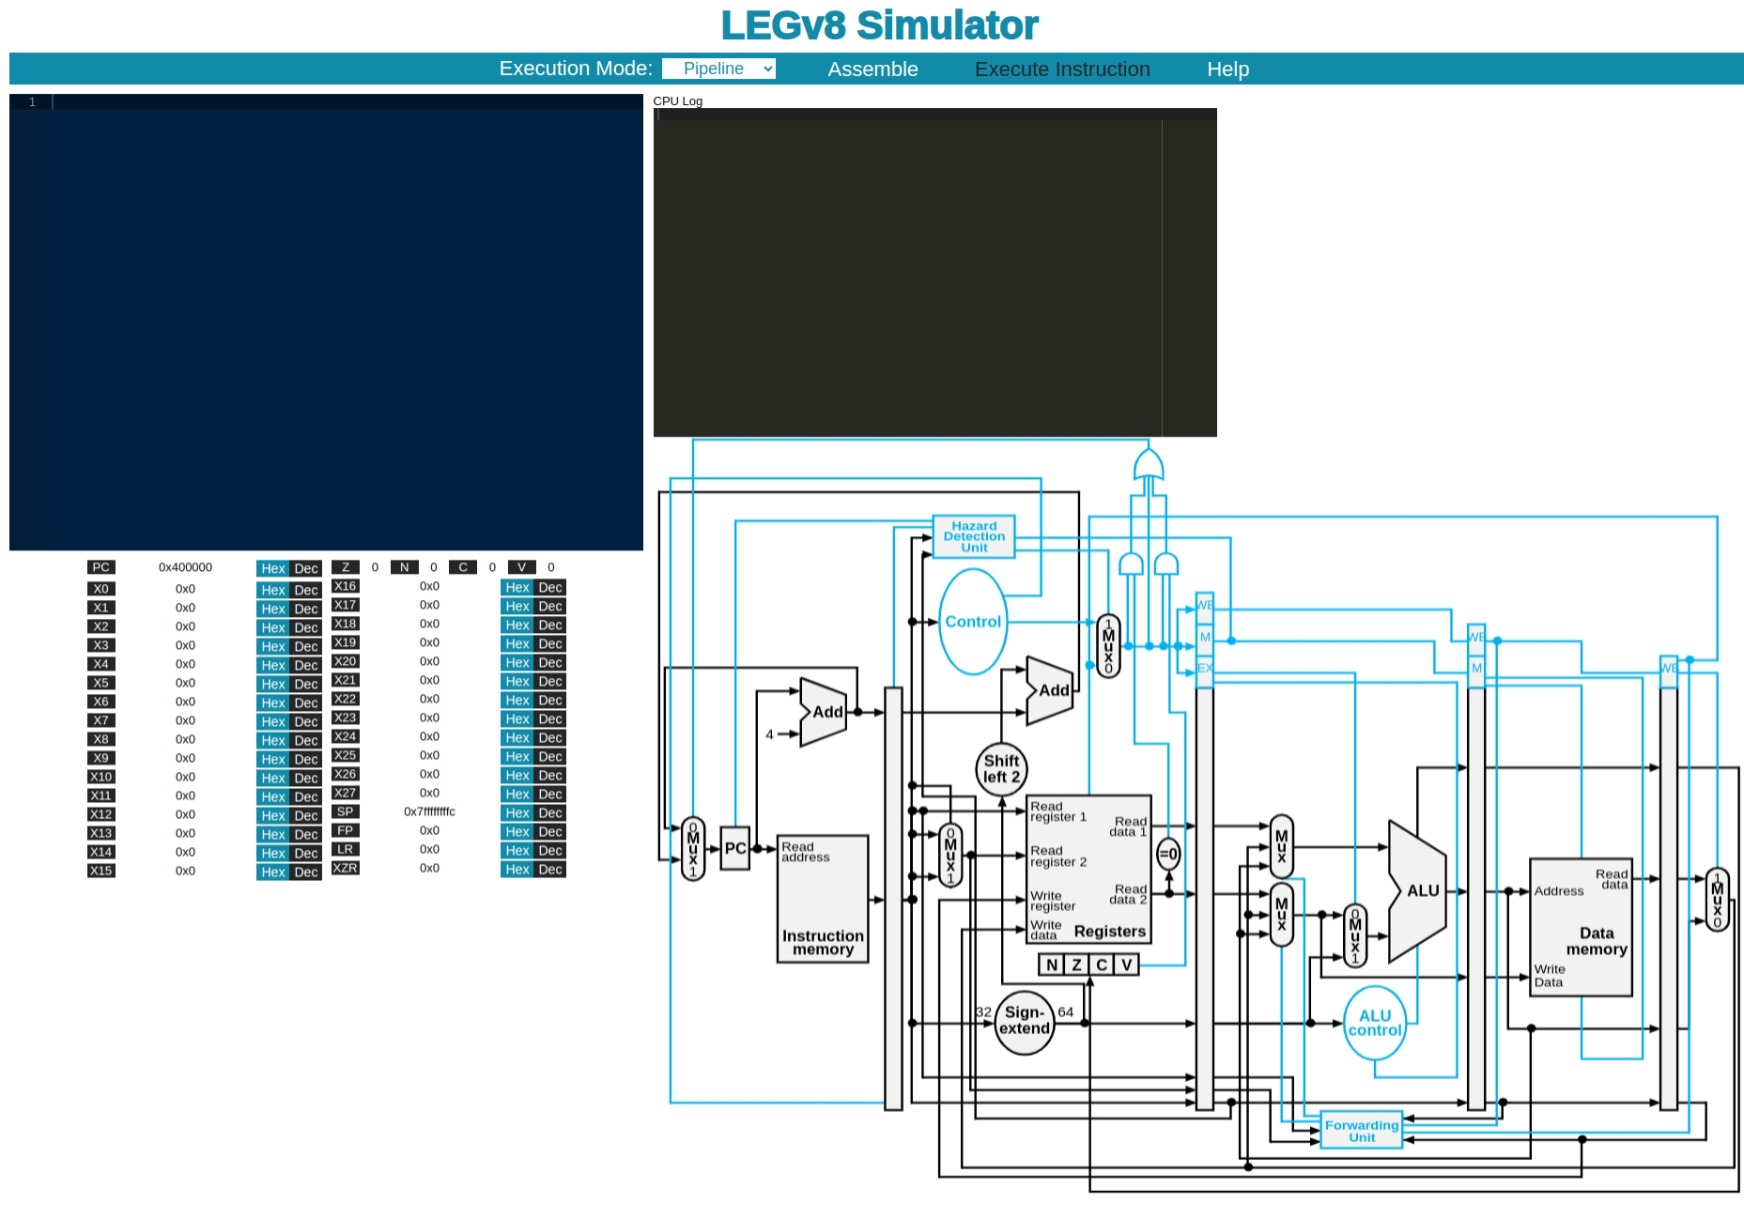
\includegraphics[width=1\linewidth]{img/old_pipeline.jpeg}
    \caption{The pipeline view}
    \label{fig:ogpipelineview}
\end{figure}
The single cycle view is comprised of a text editor on the upper left, a visualization of the \verb|PC| register, flag registers, and \verb|X| registers just below it, and a reproduction of the LEGv8 logical diagram as previously reported in Figure \ref{fig:legv8logicdiag}. The text editor is the UI component responsible for the input of LEGv8 code. It also functions as a way to present errors to the user by showing tooltips next to the lines containing invalid code. The visualization of the registers, with the exception of the flags, allows the user to switch between a hexadecimal and a signed integer representation of the values therein stored. Lastly, the visualization of the LEGv8's logical scheme highlights in red the sections of the datapath that are being used by an instruction when it gets executed. It also shows, on the bottom left, which instruction is being executed and with what arguments, and its encoding.
The pipeline visualization differs from the single cycle one by substituting the datapath diagram with a more complex one, showing more internal details of the pipeline, and by adding a read-only console above it that provides a textual representation of the instructions being executed and their position inside the pipeline.
The \emph{Assemble} button assembles the code written in the editor and automatically formats it with consistent indentations. If the code contains some syntactical mistakes, the assembly operation fails and the aforementioned tooltips get displayed. The editor is quite lenient and allows both uppercase and lowercase notation, and an unrestricted use of spaces and tabs.
If the code assembly is successful, the last button, \emph{Execute Instruction}, gets enabled and allows the user to manually execute each instruction one by one until the end. As previously described, at each step the visualization of the registers, of the datapath, and of the pipeline is updated accordingly.
\subsubsection{The good part}
\paragraph{}
It is clear from this description and the attached figures, that the simulator presents itself with a nice and functional UI, and provides additional feedback to the user both in the way of error management and by visualizing the datapath just like in the textbook \cite{patterson2016computer}. It is also extremely easy to execute, being a web application, and only necessitates a relatively modern web browser. This allows it to be run on a variety of devices, such as desktop computers, but also mobiles phones and tablets. Furthermore, it can be even self hosted and accessed remotely.
\subsubsection{The shortcomings}
\paragraph{}
Being the most popular LEGv8 simulator available, and being published by Arm, one would expect it to offer the best and most functional simulation. However, some glaring problems become evident after a cursory glance at its presentation and some simple code executions.
\subparagraph{The visual problems}
Although the choice of compatible devices is vast, more restrictive is the list of devices in which the web page correctly renders. The application is clearly constructed to work best on a widescreen computer monitor, and any attempts at enlarging the page or viewing it from a smaller device results in an incorrect scaling and arrangement of the various UI elements. A UI element that instead is lacking, is a visualization of the current state of the stack memory. Even though most of the results needed to show a correct execution of the code are evident from the values inside of the registers, being able to check how the stack is accessed is crucial for debugging and to better understand the inner workings of LEGv8.
\subparagraph{The simulation problems}
Trying to load or store values to the stack immediately presents a problem: the starting point of the stack pointer is not quadword aligned, and as such the program fails to assemble. Other than that, the simulator manages to work fairly well when executing a simple sequence of instructions, meaning without conditional jumps (conditional branches) nor function calls (branch and link), in single cycle mode. In pipeline mode, some combinations of instructions cause the simulation to stall, and sometimes instructions are skipped and not properly visualized. When trying to introduce code using comparisons, loops, and user defined functions, the simulator breaks and causes a number of problems. In the case of comparisons, the simulator sets the wrong flags (which are used to determine the outcome), and the processor ends up choosing the wrong branch. In the case of loops, this means exiting them prematurely. An example of this behavior can be seen in Figure \ref{fig:flagbug}. The code is designed to force the simulator to take the jump, which doesn't happen.
\begin{figure}[H]
	\centering
	\subfigure[X0 < X1]{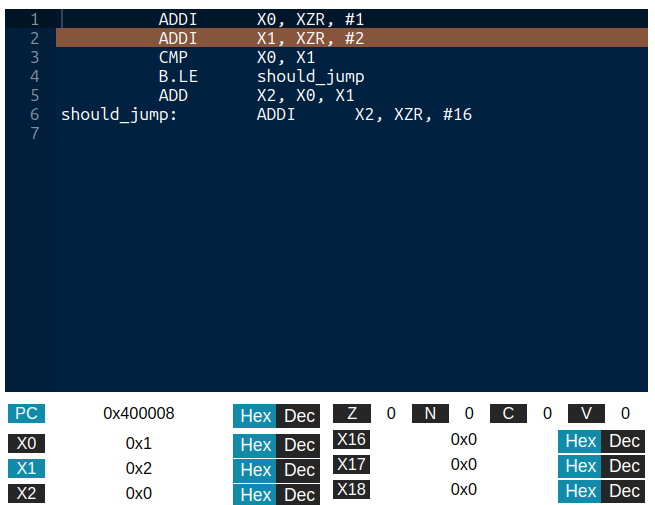
\includegraphics[width=.45\textwidth]{img/cmp_bug_1.png}}
	\subfigure[Comparison sets the flags incorrectly.]{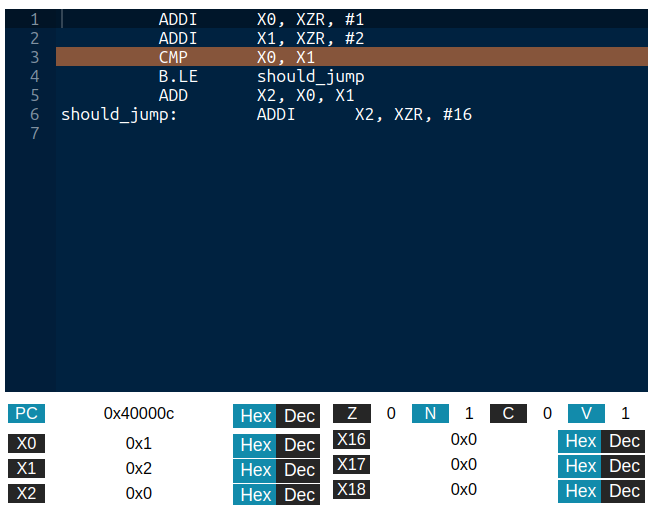
\includegraphics[width=.45\textwidth]{img/cmp_bug_2.png}}
	\subfigure[Less-or-equals jump doesn't happen.]{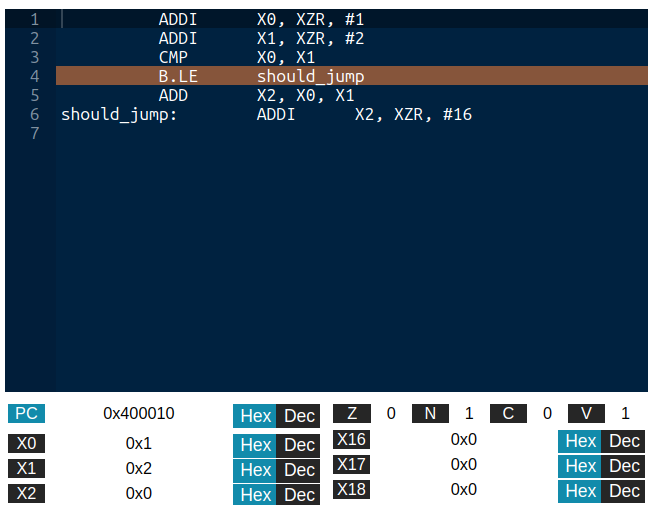
\includegraphics[width=.45\textwidth]{img/cmp_bug_3.png}}
	\subfigure[Wrong instruction executed.]{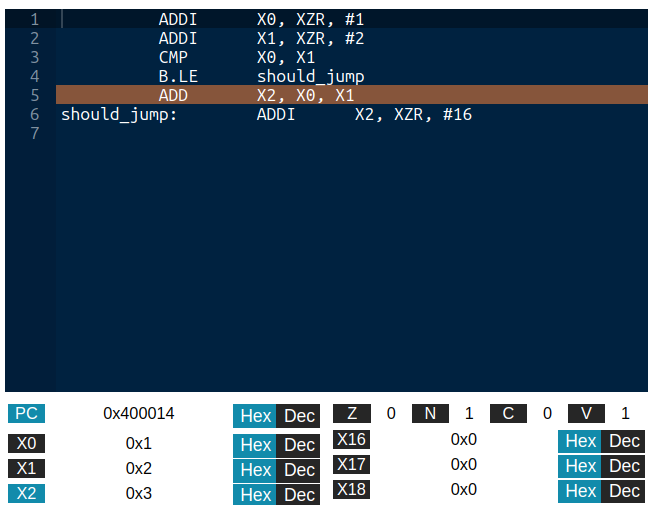
\includegraphics[width=.45\textwidth]{img/cmp_bug_4.png}}
	\caption{Comparisons do not set the correct flags and thus fail.}
        \label{fig:flagbug}
\end{figure}
The mechanism through which functions or subroutines are executed is called a \emph{branch and link} procedure. The way it works is that, when reaching the point of the code where the function is to be called, the processor saves in a certain register (the \verb|LR| register in this case) the current value of the program counter. This way, when the function has finished executing, the processor knows where to come back to resume its steps. As is evident from Figure \ref{fig:branchlinkbug}, the simulator writes the incorrect address to the \verb|LR| register, and instead of going back to where the function was called, the simulator enters the function again creating an infinite loop.
\begin{figure}[H]
	\centering
	\subfigure[BL instruction writes the incorrect address to the return register (LR).]{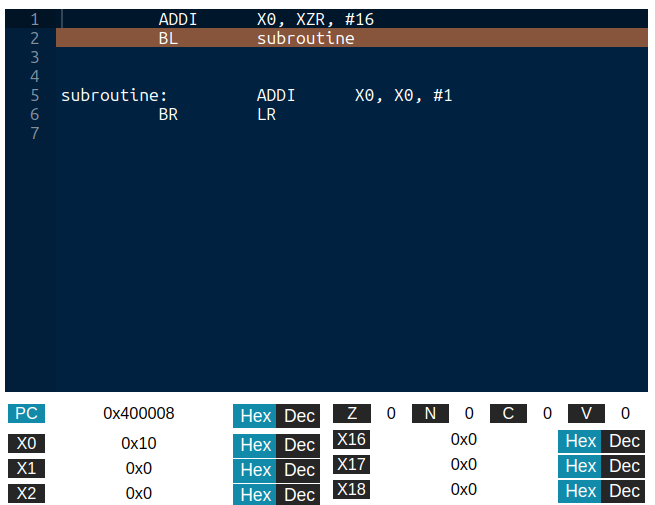
\includegraphics[width=.45\textwidth]{img/br_bug_1.png}}
	\subfigure[Jumps to the subroutine and increments X0.]{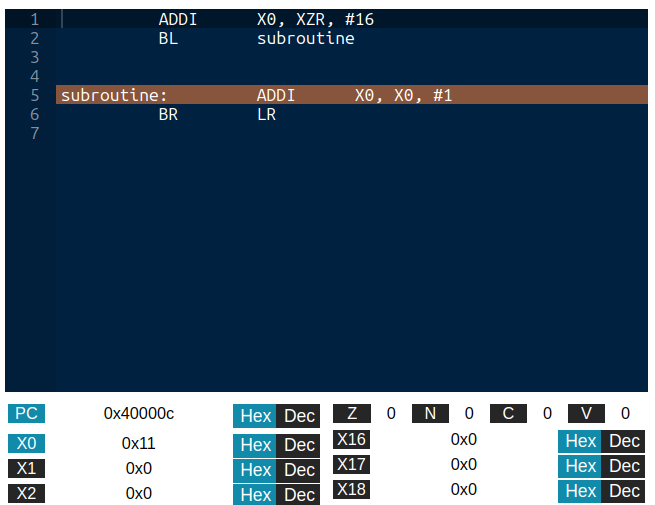
\includegraphics[width=.45\textwidth]{img/br_bug_2.png}}
	\subfigure[Reads wrong address from LR.]{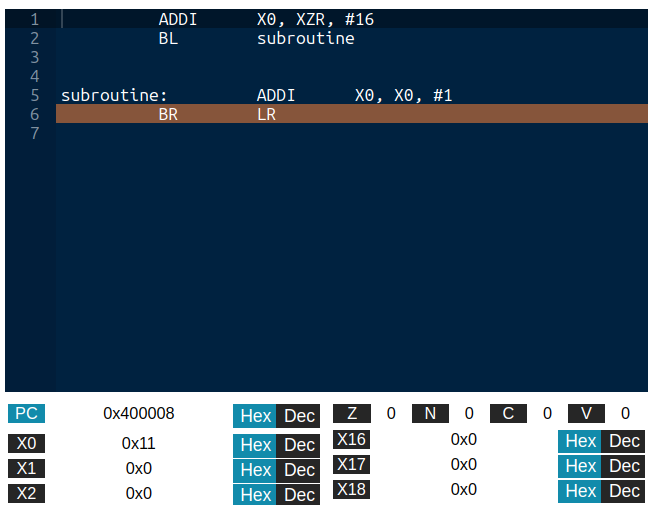
\includegraphics[width=.45\textwidth]{img/br_bug_3.png}}
	\subfigure[Returns to the start of the subroutine instead of the main program.]{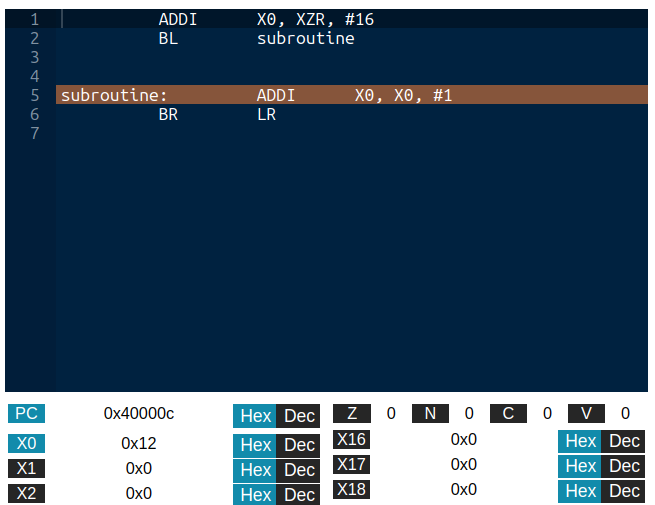
\includegraphics[width=.45\textwidth]{img/br_bug_4.png}}
	\caption{Branch returns to the wrong instruction, making it execute the branch in a loop.}
        \label{fig:branchlinkbug}
\end{figure}
\paragraph{}
Although the deficiencies in the UI could cause some annoyance, it is evident that the bugs in the simulator's logic regarding conditional branching and branch and link operations greatly limit its ability to run even the most basic examples of code.

\subsection{An inside look}\label{chap:chap1insidelook}
\begin{wrapfigure}{R}{0.3\textwidth}
	\centering
	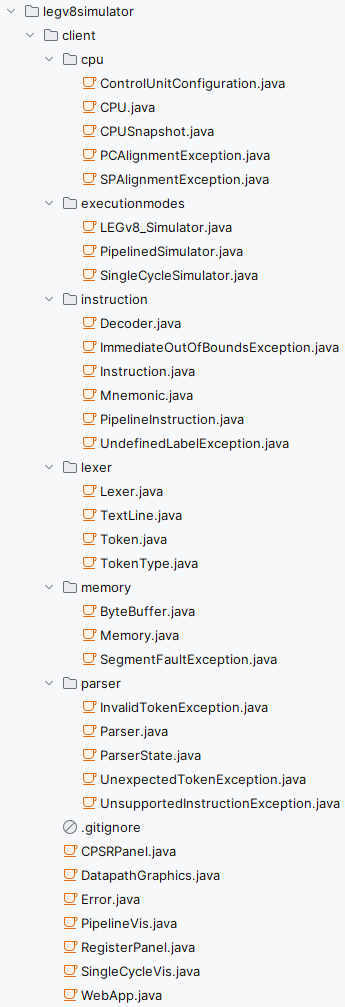
\includegraphics[width=0.30\textwidth]{img/classes.png}
	\caption{The codebase structure}
        \label{fig:codebase}
\end{wrapfigure}
\paragraph{}
Having showcased the features and criticalities of the simulator from the point of view of a casual user, it is now the time to analyze its internal logic and design choices as a developer willing to study and contribute to the project.
\paragraph{Some design choices}
Albeit deployed as a web application, the simulator is not natively written for the web, at least not its internal logic. The simulator is mostly written in Java, and uses a framework originally developed by Google called GWT \cite{gwtweb} to build from it a self-contained web application. GWT is a library that allows the creation of dynamic web applications from Java, both self-contained or using a client-server architecture. For its static components it uses normal HTML and CSS files placed in the appropriate folders, whereas for the client-side code it emulates a subset of the JVM \cite{wiki:jvm} with JavaScript. This allows the programmer to write normal Java code which will then be translated to its JavaScript equivalent and incorporated into the final web pages. The project uses version 2.7 of the library, as can be deduced from the contents of the  \verb|LEGv8_Simulator.gwt.xml| file in the source directories, and, as can be seen by the release notes \cite{gwt2.7web}, the latest Java syntax supported is Java 7.
\subparagraph{}
At the time of the simulator's development, a straightforward way to work with GWT was through the use of the Eclipse IDE \cite{web:eclipse} enhanced with the official GWT plugin \cite{web:eclipsegwtplugin}. As such, and due to the presence of Eclipse's \verb|.project| files, it is clear that the project is specifically tailored to this IDE and plugin combination.
\subparagraph{}
As we have seen from the overview of the UI, the simulator offers a featureful text editor embedded into the web page. This editor has not been developed from scratch, but has been incorporated from an existing library called AceGWT \cite{web:acegwtgit}. ``Ace'' in this case refers to an embeddable code editor for the web bearing the same name \cite{web:ace}. AceGWT is thus a Java interface built around the JavaScript-based Ace editor following the conventions specified by GWT. The end result is a GWT component that contains the Ace editor and that can be embedded into any GWT project. AceGWT in turn uses GWT version 2.8.2.
\subparagraph{}
The project uses the Eclipse's GWT plugin's way of building and deploying the web application. In this case, it all gets compiled into the \verb|/war| folder. For this reason, a separate folder containing the static resources of the website (i.e., images, HTML, and CSS files) is directly included in \verb|/war|.
\subparagraph{}
The original developers of the project have not deemed it necessary to provide a tutorial on how to build the codebase. Many things can be inferred from the structure of the project and the content of some files, but no official documentation is present anywhere in the repository.
\paragraph{The simulator's internals}
The analysis of the internal structure of the simulator will only include the Java codebase, and not the choices made regarding the web pages' style or files. Of the Java code, exception classes will not be included as they are self-describing.
The source code of the project is divided into six packages, with some classes being found inside the parent \verb|client| package, and the GWT module configuration file being located in the root \verb|legv8simulator| packages, as can be seen in Figure \ref{fig:codebase}.
\subparagraph{}
The outer classes deal with the main web application. They specify the content of the web pages and create all the GWT components that need to be rendered on the screen. Specifically:
\begin{itemize}
	\item \verb|WebApp.java| : This class contains all the code to tie together the elements of the web UI. It creates all the visual componentes and inserts them into the page. It is the entry class of the application, and the one GWT looks for the building process.
	\item \verb|SingleCycleVis.java| and \verb|PipelineVis.java|:  These two classes generate the visualization for the single cycle and pipeline datapaths. This is done by \verb|DatapathGraphics.java|, a library used to generate schematic diagrams with HTML5.
	\item \verb|RegisterPanel.java| and \verb|CPSRPanel.java|:  These two classes model the visualizations for the registers, program counter, and flag panels respectively.
	\item \verb|Error.java|:  Models the error tooltips displayed by the text editor.
\end{itemize}
\subparagraph{}
The classes inside the \verb|cpu| package are responsible for modeling the behavior of the processor, meaning the operational parts of the datapath.
\begin{itemize}
\item \verb|CPU.java| and \verb|CPUSnapshot.java|:  The \verb|CPU.java| class contains all the registers of the processor, and the ALU, implementing all the operation it is capable of performing. It fetches and decodes the instructions from the memory, communicates with it to store and load values, and performs the write back into the registers. The \verb|CPUSnapshot.java| class provides a deep copy of the \verb|CPU.java| state for use in the pipeline simulation.
\item \verb|ControlUnitConfiguration.java|:  Models the configuration of the control unit for every type of instruction.
\end{itemize}
\subparagraph{}
The \verb|memory| package is dedicated to the modelization of the main memory of the processor.
\begin{itemize}
\item \verb|ByteBuffer.java|:  A utility class used to implement a byte buffer of client specified length, used to store data in big-endian format. As specified by the author, this class has been written because emulation for \verb|java.nio.ByteBuffer| was not supported by GWT.
\item \verb|Memory.java|:  This is the class used to implement the address space of LEGv8. It follows closely Patterson's and Hennessy's specification as presented in Figure \ref{fig:legv8memdiag} , and as such it appears like a single array of bytes. In this case it's implemented via a \verb|HashMap<Long, Byte>| and offers various methods to read and write different amounts of bytes to it.
\end{itemize}
\subparagraph{}
The \verb|instruction| packages contains all the classes necessary to model the concept of an instruction as described by Patterson and Hennessy.
\begin{itemize}
	\item \verb|Instruction.java| and \verb|PipelineInstruction.java|: These two classes model an instruction. An instruction contains its mnemonic, its arguments, its control signals for the control unit, and its position inside of the source code. The \verb|PipelineInstruction.java| class is a wrapper for \verb|Instruction.java| and is used in the pipelined execution.
	\item \verb|Mnemonic.java|: An enumerator class containing the name, OPcode, type, and ALUcode of all of the implemented instructions.
	\item \verb|Decoder.java|: This class is responsible for taking the tokenized source code from the parser, and converting each line into a valid instruction. 
\end{itemize}
\subparagraph{}
The \verb|lexer| and the \verb|parser| packages, although separate, can be considered as a single entity. Their purpose is to take the code written inside the web editor and perform various steps to verify its correctness and produce a tokenized version to be used later for the decoding of the instructions.
\begin{itemize}
    \item \verb|Lexer.java|: The class responsible for scanning the code line by line and tokenizing it. The \verb|TextLine.java| class models a single line of code, the \verb|Token.java| models a token, and the \verb|TokenType.java| is an enum class containing the corresponding regular expressions to tokenize each part of the line of code.
    \item \verb|Parser.java|: The class responsible for checking the validity of LEGv8 code by passing each line's tokens obtained by the lexer through a finite state machine defined by \verb|ParserState.java|, whose structure can be seen in Figure \ref{fig:oldparser}.
\end{itemize}
\begin{landscape}
    \begin{figure}[H]
	\centering
	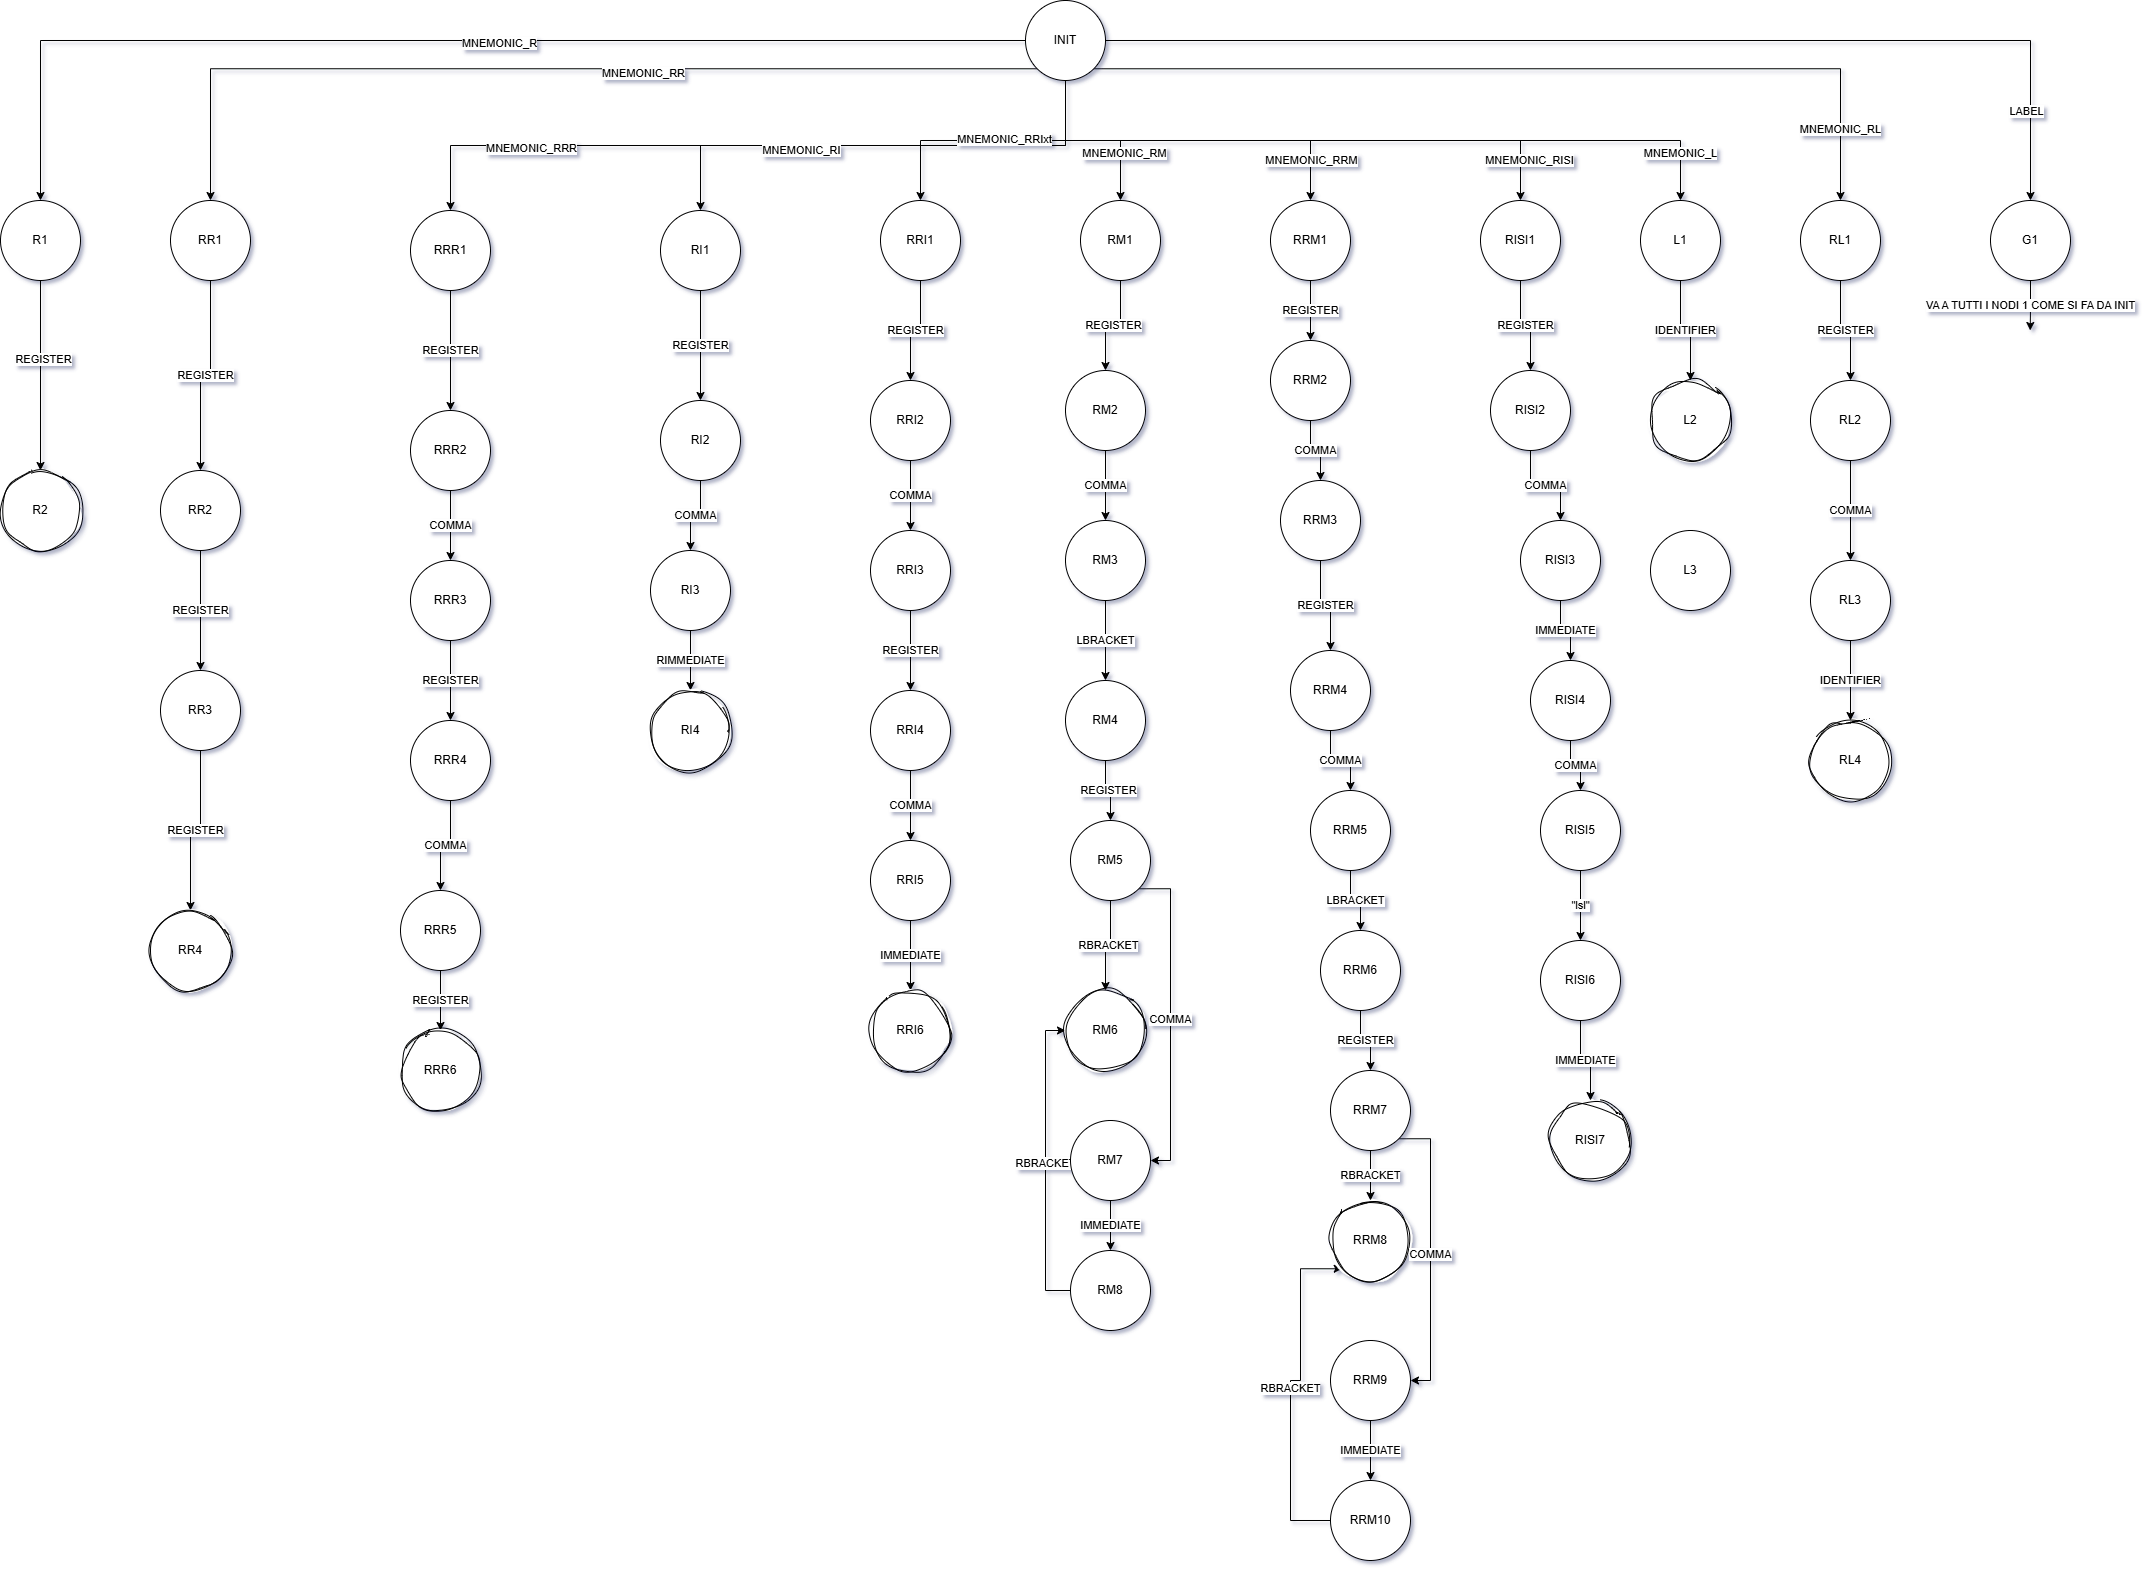
\includegraphics[width=1.25\textwidth]{img/parser_diagram.png}
	\caption{Diagram of the parser's states}
        \label{fig:oldparser}
\end{figure}
\end{landscape}
\subparagraph{}
Lastly, the \verb|executionmodes| package contains the logic necessary to initialize the simulator and being the execution through either a single cycle or pipelined mode.
\begin{itemize}
	\item \verb|LEGv8_Simulator.java|: The abstract class responsible for setting up the simulation, initializing the various components of the processor, and signalling the CPU when to perform the various stages of the LEGv8 execution pipeline.
	\item \verb|SingleCycleSimulator.java| and \verb|PipelinedSimulator.java|: These two classes extend \verb|LEGv8_simulator.java| and are responsible for making the proper adaptations to the code to fit the respective execution mode.
\end{itemize}
\paragraph{}
Now that this brief overview of the codebase has come to an end and some context has been provided, we will conclude the chapter by discussing the positives and negatives of the internal design choices of the simulator, and in the end explaining the motivations for choosing it as the subject of this thesis' work.
\paragraph{The good}
The simulator is written in Java, which makes it easy to structure, extend, and fix thanks to its high level design, and offers quality of life improvements in the form of the Java library to expedite development. Being deployed as a web application, it makes it compatible with most devices currently available and executable in a few clicks with most browsers. Furthermore, GWT allows the developers to focus on a single programming language without worrying too much about the complications of web programming. The codebase is fairly well structured with extensibility in mind, and most functions of the simulator reside in the correct packages and classes. With the exceptions of the two bugs previously mentioned, the instructions are executed correctly and the simulator works properly.
\paragraph{The bad}
The bugs plaguing the current iteration of the simulator can be easily spotted inside the codebase, but without a way to compile it into a working application they remain unfixed. The simulator does not implement the entirety of the LEGv8 ISA, and as such, even though its structure is apt for extension, the logic is designed to work with integer registers, values, and instructions. Eclipse, although featureful, is not the most advanced IDE to work with and doesn't offer any real advantages over the others. The pipelined execution mode has not been completed and is not well structured, which causes problems in identifying its issues and extending it with new features. 
\paragraph{And the ugly}
GWT is an extremely old library for creating web applications. It has been abandoned by Google and is now maintained by the community through infrequent updates. The version used in the project uses an outdated build system that is being abandoned by the newer versions of the library, and strongly limits the Java features that can be used in the project. Similarly, AceGWT is a one-off library that is not being actively updated with newer versions of the Ace editor nor GWT. It is a crucial dependency of the project and would require parallel efforts to bring it up to current standards. Because of GWT and its outdated build process, the project is deeply coupled with the Eclipse IDE and its configuration has been slightly customized from the default one since it's a client-only application. Furthermore, newer releases of the Eclipse IDE (newer than 2023-09) break the installation of the GWT plug-in because of a change in libraries, making it impossible to develop with it. Certain features of the codebase, such as the datapath visualization for example, are complex and very sparsely documented, making it difficult to follow their logic. The single cycle mode was developed before the pipeline version, with the latter being adapted on top of the former later on. For this reason, it doesn't feel like the simulator is truly executing the pipeline stages individually, and this contributes to the instability of this execution mode.
\section{Motivations for choosing Arm's simulator}
\paragraph{}
Although the simulator presents some criticalities both from the point of view of the end user and the developer that leave it in a barely working state, we feel that its general structure, presentation, and prominence in the LEGv8 landscape make it stand out as the most impactful project to work on, and, when considering the work to be done, give it the prospect of being the most feature complete LEGv8 simulator available.
\paragraph{}
Not all the issues raised in this final section of the chapter have been tackled by this thesis' work. For example, the pipelined mode and the general structure of the codebase have been mostly left untouched, and, save for a few enhancements to the UI, improvements to the HTML and CSS have not been taken into consideration. Nonetheless, in the following chapters we will present the work done to restore the simulator to a working state and to enhance it to the point of providing a full simulation of the LEGv8 ISA, at least where single cycle mode is concerned.